\section{系统交互}
我们在设计系统时，力求将master参与所有操作的程度降至最低。在此
背景下，下面将说明客户端、master和chunkserver如何交互，以实现数据
mutation、原子\textbf{record append}和\textbf{snapshot}。

\subsection{lease与mutation顺序}
mutation是一种会改变某个chunk的内容或元数据的操作，例如普通写入或追加操作。
每个mutation都会在该chunk的所有副本上执行。我们使用lease来在各个副本之
间维持一致的mutation顺序。master会把某个chunk的lease grant给其中一个副本，
我们称这个副本为primary。primary会为该chunk上的所有mutation选择一个串行顺序。
所有副本在应用mutation时都遵循这个顺序。因此，全局mutation顺序首先由master选择的
lease顺序决定；在同一个lease内，则由primary分配的序列号决定。

lease机制旨在降低master的管理开销。lease的初始超时时间为60秒。不过，
只要chunk仍在发生mutation，primary就可以向master请求延期，并且通常
能够无限期获得延期。这些延期请求和grant lease会捎带在master与所有
chunkserver定期交换的HeartBeat消息中。master有时会尝试在lease
到期前撤销它(例如，master希望禁止对一个正在重命名的文件进行mutation时)。
即使master失去了与某个primary的通信，它也可以在旧lease到期后，
安全地向其他replica grant lease。\emph{(译者注：这里的rename更准确地说
是master对namespace映射的一次原子修改，
即把某个文件对象从旧路径绑定到新路径，而不是复制或重建文件数据。
由于GFS client可能缓存了chunk的primary/replica信息，并在已有lease
有效期内绕过master继续向primary发起append/write，master如果希望
rename成为一个清晰的发布/提交边界，就需要暂时禁止该文件上的mutation。
因此它可能在lease到期前主动revoke lease，使基于旧缓存状态的写入失效，
后续写入必须重新联系master，并基于新的namespace状态重新获得授权。你看
假如你已经rename成功了，但是去append原来的那个文件路径才是ok，岂不奇怪？)}

Figure 2通过以下带编号的步骤，展示了一次写入操作的控制流。

1. 客户端询问master：哪个chunkserver持有该chunk当前的lease，以及
   其他replica的位置。如果没有任何replica持有lease，master会向
   它选择的一个replica grant lease(此步骤未在图中展示)。

2. master返回primary的身份以及其他secondary replica的位置。客户端会
   缓存这些数据以供之后的mutation使用。只有当primary不可达，或回复
   表示自己不再持有lease时，客户端才需要再次联系master。

3. 客户端将数据推送到所有replica。推送顺序可以任意。每个chunkserver
   都会将数据保存在内部LRU缓冲区缓存中，直到数据被使用或因老化而
   被逐出。通过将数据流与控制流解耦，我们可以不受哪个chunkserver
   是primary的影响，依据网络拓扑调度开销较大的数据流，从而提升性能。
   section3.2会进一步讨论这一点。

4. 所有replica确认收到数据后，客户端向primary发送写请求。该请求标识
   先前已推送到全部replica的数据。primary为它收到的所有mutation分配
   连续序列号\emph{(译者注：master元数据的mutation顺序号/
   operation log顺序和每个chunk内data mutation的顺序是两套不同的顺序体系，
   不能混为一个全局序列)}，这些mutation可能来自多个客户端，从而提供所需的串行化。
   它按照序列号顺序将mutation应用到自己的本地状态。

5. primary将写请求转发给所有secondary replica。每个secondary replica都按照
   primary分配的相同序列号顺序应用mutation。

6. 所有secondary都会回复primary，表明自己已完成该操作。

7. primary回复客户端。任一replica遇到的错误都会报告给客户端。发生错误时，
   写入可能已经在primary和任意一个secondary replica子集上成功。(如果它
   在primary处失败，就不会获得序列号，也不会被转发。)
   客户端请求会被视为失败，修改后的区域则处于不一致状态。我们的客户端
   代码会通过重试失败的mutation来处理这类错误。它会先对步骤3到步骤7进行
   若干次尝试；若仍失败，便从写入操作的开始处重新重试。
   \\\begingroup\itshape 译者注：可以考虑一种网络隔离场景来理解该机制。
   \\假设chunk有A、B、C三个replica，当前版本号为7，A持有lease并作为primary。
   此时A与master、B、C发生网络隔离，但client仍能连接到A。client可能仍基于旧
   缓存认为A是primary，并向A发起mutation。A即使能在本地为该mutation
   排序并尝试执行，也无法把该mutation转发给B、C并获得它们的确认，因此该请
   求会被报告为失败；如果mutation只在部分replica上执行成功，则被修改
   区域处于inconsistent状态，client需要重试。

   随着A与master失联，master在旧lease过期后，可以从仍然可达且
   up-to-date的replica中选择新的primary，例如B，并推进chunk version number，
   例如从7增加到8。B、C收到新版本后继续参与后续mutation；
   A因为错过了版本更新和后续mutation，恢复后会被master识别为
   stale replica，不会再被返回给client，
   也不会参与新的mutation，之后会被垃圾回收。

   这里的关键不是多数派提交，而是：同一个chunk的mutation必须由当前有效
   lease holder排序，并由所有参与的replica按相同顺序执行；旧primary的
   lease到期后不能继续合法提交mutation，版本号则用于识别那些错过mutation
   的stale replica。
   
   这里还有一个特别关键的点，version更准确地说是chunk的一个epoch标签。
   master会用version判断哪些replica属于当前有效的副本。一次mutation需要由
   当前lease holder排序，并由master当前认可的up-to-date replicas按相同顺序执行。
   如果某个replica在version推进期间不可用，它恢复后因版本落后而被识别为stale，
   不再参与后续mutation。简单理解，version隐式蕴藏了一个“有效replica”列表，
   一次成功的mutation必须让这列表里的所有人都执行mutation。
   \endgroup

如果应用程序的写入很大，或跨越了chunk边界，GFS客户端代码会将其拆分为
多个写入操作。它们都会遵循上述控制流，但可能与其他客户端的并发操作
交错，并被其覆盖。
因此，这个共享的文件区域最终可能包含来自不同客户端的片段。不过，各replica仍然
相同，因为每个单独操作都以相同顺序在所有replica上成功完成。正如
section2.7所述，这会使文件区域处于consistent但undefined的状态。

\begin{figure}[t]
  \centering
  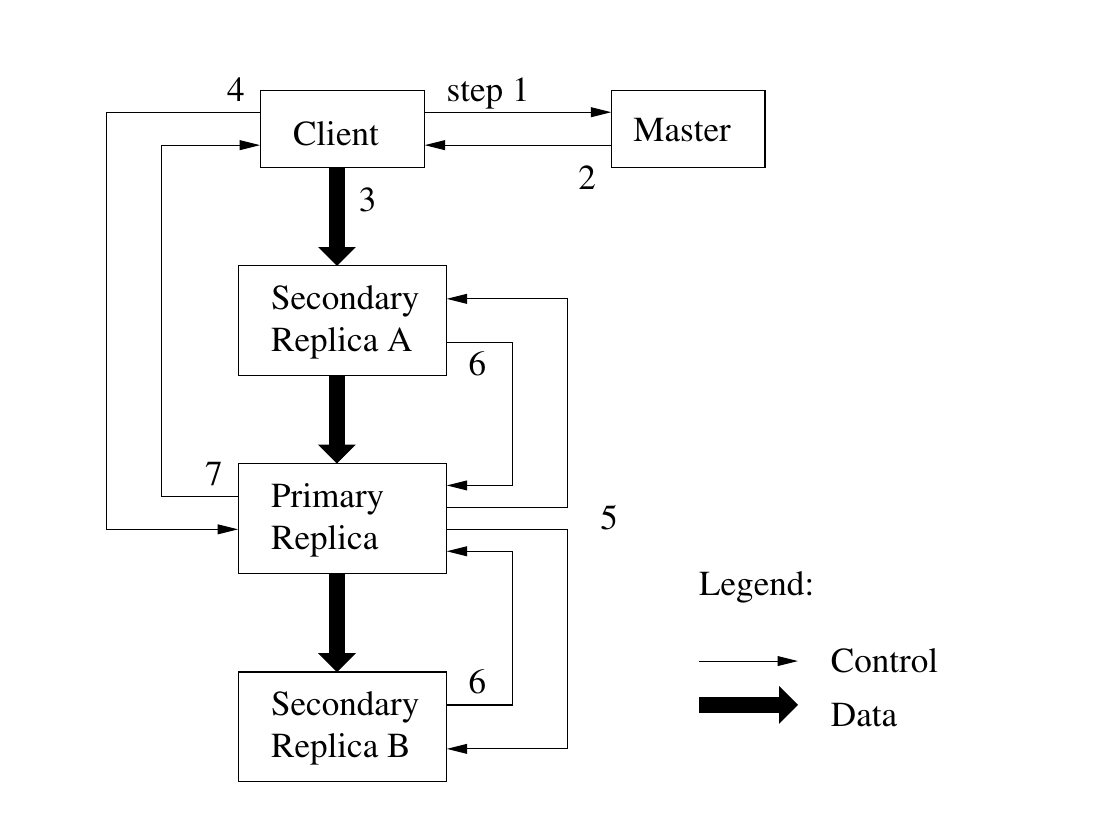
\includegraphics[width=0.95\columnwidth]{figures/original/gfs-figure-2-write-control-data-flow.png}
  \captionsetup{justification=centering}
  \renewcommand{\figurename}{Figure}
  \caption{写入控制流和数据流}
  \label{fig:gfs-write-control-data-flow}
\end{figure}

\subsection{数据流}
我们将数据流与控制流解耦，以高效利用网络。控制流从客户端流向
primary，再流向所有secondary；而数据则以流水线方式，沿着精心选择的
chunkserver链线性推送。我们的目标是充分利用每台机器的网络带宽，避免
网络瓶颈和高延迟链路，并尽量缩短推送全部数据所需的延迟。

为了充分利用每台机器的网络带宽，数据会沿着一条chunkserver链线性
推送\emph{(译者注：例如Client->A->B->C)}，而不是以其他拓扑结
构(例如树形结构)分发。这样，每台机器的全部
出站带宽都会用于尽快传输数据，而不是把出口带宽分摊给多个接收者\emph{(
译者注：一台机器的出口宽带是有限的。实际上别的场景上，Fan-Out在架构上一般
不是什么好设计，译者在实际的工程中，例如IM群聊场景也有这样的体会，
Fan-Out架构会让群聊发送接口成为瓶颈——大量的CPU损耗和网络开销)}。

为了尽可能避开网络瓶颈和高延迟链路(例如交换机之间的链路通常同时具备
这两个问题)，每台机器都会将数据转发给网络拓扑中距离最近、且尚未收到
数据的机器。假设客户端正在向chunkserver S1到S4推送数据，它会先将
数据发送给最近的chunkserver，例如S1。
S1会将数据转发给S2到S4中距离自己最近的chunkserver，例如S2。类似地，
S2会将数据转发给S3或S4中距离S2更近的一个，如此继续。我们的网络拓扑
足够简单，因此可以根据IP地址准确估计这些“距离”。

最后，我们通过在TCP连接上对数据传输进行流水线化来降低延迟。一旦
chunkserver收到一部分数据，就会立即开始转发。流水线对我们特别有用，
因为我们使用具有全双工链路的交换网络。立即发送数据不会降低接收速率。
在没有网络拥塞时，向R个replica传输B字节数据的理想耗时为B/T+RL，其中T
是网络吞吐量，L是字节在两台机器间传输的延迟。我们的网络链路通常为
100Mbps(T)，而L远小于1ms。因此，理想情况下，分发1MB数据大约需要
80ms。

\subsection{原子\textbf{record append}}
GFS提供了一种称为\textbf{record append}的原子追加操作。在传统写入中，
客户端指定数据要写入的offset。对同一区域的并发写入无法串行化：该区域
最终可能包含来自多个客户端的数据片段。
而在\textbf{record append}中，客户端只指定数据。GFS会在它选择的offset处，
\textbf{至少一次}原子地将数据追加到文件中(即作为一段连续字节序列)，
并将该offset返回给客户端。这类似于在Unix中向以O\_APPEND模式打开的文件写入
数据，即使是多个writer并发写入，也不会出现竞争而产生的“交叉文本”。
\\\emph{(译者注：这里作者实际是在说Unix O\_APPEND文件写入和GFS
的record append语义相似，都是原子追加。然而，其实GFS的语义又
和Unix O\_APPEND不完全一样。第一点是GFS的record append保证的是
\textbf{至少一次}，也就是两个线程并发追加内容，一个写hello，一个写world，
那么真实在GFS里面的内容可能是hellohelloworld，或者helloworldhelloworld。
你看，它虽然保证了一个record原子被插入，但是是多少次呢？答案是GFS只保证一次。而且
最需要注意的是，插入后也许在chunk server不同的机器上读，会读出不同的结果。
这里埋下伏笔，我将在后续提到这个badcase。这个“乱序问题”很微妙，但是也可以被解决)}

\textbf{record append}被我们的分布式应用大量使用：不同机器上的许多客户端会并发向同一
文件追加数据。如果使用传统写入，它们就需要额外进行复杂且昂贵的同步，
例如通过分布式锁管理器完成同步。在我们的工作负载中，这类文件通常充当
多生产者/单消费者队列，或保存来自许多不同客户端的合并结果。
\\\begingroup\itshape
译者注：

例如chunk10是文件的最后一个chunk，primary是server A。
客户端尝试向该chunk执行record append时，如果A发现该chunk的剩余空间
不足以容纳完整record，GFS不会把这条record拆开跨chunk存放，而是由A
将chunk10的剩余部分填充为padding，并通知其他副本执行同样的padding mutation。
随后客户端需要在下一个chunk上重试record append——也就是客户端需要请求master，
找master创建下一个chunk的元信息。

这里体现了GFS record append的一个设计取舍：为了保证一条record作为连续字节序列
原子地落在某个chunk内，GFS接受了chunk边界处可能产生padding和重试的代价。
由于GFS写入流程是先push data到各副本，再请求primary执行mutation，
当大量客户端并发append且当前chunk接近满时，可能会出现一批已经push到旧chunk
但最终无法写入的无效数据传输。

不过，这不意味着GFS不支持多生产者追加。相反，GFS的record append正是为了支持
多个客户端并发向同一文件追加记录。但单个文件的当前active chunk只有一个primary
负责排序和分配offset，因此单文件写入吞吐不能随着writer数量线性扩展。若需要更高
写入吞吐，通常应采用分片输出或多个队列文件，而不是让所有producer写入同一个文件。
\endgroup

\textbf{record append}是一种mutation，它遵循section3.1中的控制流，只是在primary处
增加了一些额外逻辑。客户端将数据推送到文件最后一个chunk的所有replica，
然后向primary发送请求。primary会检查：在当前chunk执行\textbf{record append}是否会使
其超过最大大小(64MB)。
如果会超过，primary会将chunk填充到最大大小，通知secondary执行相同操作，
并回复客户端，表示应在下一个chunk上重试该操作。(\textbf{record append}被限制为至多
最大chunk大小的四分之一，以将最坏情况下的碎片控制在可接受范围内)。
如果\textbf{record}能够容纳在最大大小内(这是通常情况)，primary会将数据追加到自己
的replica中，通知secondary在与primary完全相同的offset写入数据，最后向
客户端回复成功。

如果\textbf{record append}在任一replica上失败，客户端会重试该操作。因此，同一chunk的
replica可能包含不同数据，也可能全部或部分包含同一\textbf{record}的重复内容。GFS并不
保证所有replica在字节层面完全相同；它只保证数据至少会作为一个原子单元被
写入一次。
这一性质直接来自一个简单事实：要让操作报告成功，数据必须已在某个chunk
的所有replica上的相同offset处被写入。并且在此之后，所有replica的长度至少会
达到\textbf{record}结尾。因此，即使之后由不同replica成为primary，任何未来\textbf{record}都会
被分配到更高的offset，或被分配到不同chunk。
按照我们的一致性保证，成功的\textbf{record append}操作写入数据的区域是已定义的
(因此也是一致的)，而其间的区域则是inconsistent的(因此也是未定义的)。正如
section2.7.2所讨论的，我们的应用可以处理inconsistent区域。
\\\emph{译者注：回收之前的伏笔。读者可以去看Youtube观看Raft2020 Lec3 GFS视频，
在1h10分处它讲解了一个由于失败重试，导致的“乱序问题”，它是一个很神奇的badcase。
\\在真实的应用中，我们会使用append record
来做追加的数据写入，读取则是从头读到已consistent的区域，然后从头到尾扫描“自标识”特征来识别record
——这样可以剔除无用padding或者record之间的garbage信息。但是这里教授的例子
很微妙，它描述了一种非常奇妙的现象：多个writer append record同一个GFS File时，假如一次写入尝试因为
“只有部分replica成功append”而失败，后续客户端重试，会留下“脏数据”，而这个脏数据也是合理的自标识数据。
因此，就算业务层自己做了record自标识识别，也做了去重，但是在不同的机器可能会消费到不同的record顺序。
所以怎么解决呢？一是可以干脆就不让多人写一个GFS文件了，事实上HDFS就是这么做的，它将lease做到了客户端和
master上，保证同时只有一个客户端向一个文件append；二是可以改造GFS，我可以提供一些想法：可以尝试
让所有机器都成为primary的复制状态机，每当primary上任的时候，强制让其它secondary同步自己经历过的mutation，
不允许出现分岔。读者可以多思考思考复制状态机以及Raft的No-op Entry优化，从这两个角度入手改造GFS。}

\subsection{\textbf{snapshot}}
\textbf{snapshot}操作几乎可以瞬时创建一个文件或目录树(即“source”)的replica，同时尽量
减少对正在进行的mutation的干扰。用户使用它快速创建超大数据集的分支
replica(并且经常递归地创建这些replica的replica)，或在试验某些之后可轻松提交
或回滚的修改前，对当前状态创建检查点。

与AFS[5]类似，我们使用标准的\textbf{copy-on-write}技术实现\textbf{snapshot}。当master收到\textbf{snapshot}
请求时，首先会撤销即将创建\textbf{snapshot}的文件中所有chunk尚未到期的lease。这样
可以确保之后对这些chunk的任何写入，都必须与master交互以找到lease持有者。
这使master有机会先创建该chunk的新replica。

待lease被撤销或到期后，master会将该操作记录到磁盘。然后，它通过复制
source文件或source目录树的元数据，将这条日志记录应用到内存状态中。新创建的
\textbf{snapshot}文件与source文件指向相同的chunk。

在\textbf{snapshot}操作之后，客户端首次想要写入chunk C时，会向master请求当前lease
持有者\emph{(译者注：举个好例子，假如正在append，客户端对primary有所缓存，但是在此
刻chunk lease被收回，客户端写入时会发现not primary，此时会去请求master寻找新的primary)}。
master发现chunk C的引用计数大于1。它会暂缓回复客户端请求，
转而选择一个新的chunk handle C'。随后，它要求每个持有C当前replica的
chunkserver创建一个名为C'的新chunk\emph{(译者注：lease是master调用chunkserver
实现的，笔者认为创建C'时可以夹带copy-on-write信息，通知它进行复制)}。
通过在与原chunk相同的chunkserver上创建新chunk，我们确保数据可以在
本地复制，而无需经由网络传输(我们的磁盘速度大约是100Mb以太网链路的
3倍)。从此以后，请求处理与任何普通chunk都没有区别：master将新chunk C'的lease grant给
其中一个replica，然后回复客户端。客户端随后可以像平常一样写入该chunk，
而不会察觉它刚刚是从一个现有chunk创建出来的。
\\\emph{译者注：snapshot在用户视角那里其实就是像拷贝了一个文件夹，但是这个拷贝
特别快，该文件夹下面的所有文件的所有chunk lease都会被revoke掉。读者可能会担心
这里会有惊群效应客户端来拿lease会引发惊群效应。可以这样考虑：
1.读客户端不需要lease，只有正在写的客户端需要来重新拿；2.用户可以选择只snapshot
一个小文件夹，尽量避免snapshot整个目录树，避免惊群。}
